\providecommand{\main}{../..}
\documentclass[\main/main.tex]{subfiles}

%\graphicspath{ {\main/chapters/circuiti/}}


\begin{document}
\section{Tema d'esame 31 gennaio 2018}
\subsection{Testo del esame}
\subsubsection{Esercizio 1}
Siano $IN_1,IN_2$ dei segnali digitali compresi tra $0$ e $3.3V$ e $A$ un segnale digitale compreso tra $0$ e $5V$.



\begin{center}
    \begin{circuitikz}
        \draw(-2,3) node[left] {$IN_1$} (-2,3) to[short, o-](-1,3);
        \draw(-1,3) to[Tnmos, l=$N_1$](0,3);
        \draw (-0.5,4) node[above] {$A$};
        \draw (0,3) -- (1,3) -- (1,1);

        \draw(-1,1) to[Tnmos, l=$N_2$] (0,1);
        \draw (-0.5,2) node[above] {$\neg A$};
        \draw (0,1) -- (1,1);
        \draw(-1,1) -- (-2,1) node[left] {$IN_2$};

        \draw (1,2) to[short, *-] (2,2) node[above] {$V_{out}$} (2,2) to[capacitor = C](2,0) node[ground]{} (2,0);
    \end{circuitikz}
\end{center}



\[K_n = 0.5 \frac{m A}{V^2}\]
\[V_{t,n} = 0.7V\]
\[C = 0.5pF\]

\begin{enumerate}
\item Determinare i valori (Logici e di Tensione) assunti dall'uscita $V_{out}$ quando $A = "1"$ e quando $A = "0"$ in funzione dei valori degli ingressi.
\item Agli Ingressi $A$ e $IN_1$ e' applicata un' onda quadra a frequenza $1MHz$ e all' ingresso $IN_2$ un' onda quadra a frequenza $500KHz$. Si consideri il fronte di salita dei due segnali allineato. Disegnare l'andamento temporale di $V_{out}(t)$ e calcolare la potenza dinamica dissipata dal circuito.
\item Calcolare il tempo di commutazione della porta logica quando gli ingressi passano $IN_1=0,IN_2=1,A=0 \longrightarrow IN_1=0,IN_2=0,A=1$ (si noti il funzionamento in zona ohmmica).
\end{enumerate}

\clearpage
\subsubsection{Esercizio 2}
Si consideri il circuito in figura. I diodi hanno una tensione di accensione $V_\gamma = 0.7V$

\begin{center}
    \begin{circuitikz}
        \draw (-4,6) to[american voltage source, v^<= $V_{IN}$] (-4,0) node[ground] {};
        \draw(2,6) to[short, -*] (0,6) to[short] (0,6) to[R,l_=$R_3$] (-4,6);
        \draw(0,4) to[diode,l_=$D_1$] (0,6);
        \draw(2,6) to[diode,l=$D_2$] (2,4);
        \draw(0,4) to[R,l=$R_1$] (0,2);
        \draw(0,2) to[short, *-*] (2,2);
        \draw(2,4) to[R,l=$R_2$] (2,2);
        \draw(0,2) to[C,l=$C_1$] (0,0)  node[ground]{} (0,0);
        \draw(2,2) to[C,l=$C_2$] (2,0)  node[ground]{} (2,0);
    \end{circuitikz}
\end{center}

\[R_1 = 250 \Omega\]
\[R_2 = 100 \Omega\]
\[R_3 = 50 \Omega\]
\[C_1 = C_2 = 10 \mu F\]

\begin{figure}[H]
    \center
    \begin{tikzpicture}
      \draw[->] (-0.5,0) -- (8,0) node[right] {$t$};
      \draw[->] (0,-3) -- (0,3) node[above] {$V_{in}$};
      \draw[thick](0,2) -- (2,2) -- (2,-2) -- (4,-2) -- (4,2) -- (6,2) -- (6,-2) -- (8,-2);
      \draw[dotted] (2,-2) -- (0,-2);
      \draw(0,2) node[left]{+10V};
      \draw(0,-2) node[left]{-10V};


    \end{tikzpicture}
\end{figure}


Attraverso il generatore ideale di tensione $V_{in}$ viene applicata al circuito un'onda quadra di livelli $-10V,+10V$ con frequenza $10Hz$ come in figura.

\begin{enumerate}
\item Tracciare su di un grafico quotato l'andamento della tensione al nodo $V_x$ dal tempo $t=0s$ al tempo $t=200ms$ e calcolare il valore della costante di tempo $\tau$ per sia il fronte di salita e sia quello di discesa
\item A causa di un malfunzionamento la capacita' $C_1$ esplode diventando un corto circuito. Se il generatore $V_{in}$ rimane acceso, quale dei due diodi deve dissipare piu' potenza? Calcolarne il valore.
\item La Capacita' $C_1$ viene in seguito sostituita con una resistenza $R = 150 \Omega$ mentre la capacita' $C_2$ e' ancora presente. In queste condizioni, Tracciare nuovamente l'andamento della tensione al nodo $V_x$ dal tempo $t = 0s$ a $t = 200ms$ su di un grafico quotato e calcolare i nuovi valori delle costanti di tempo.
\end{enumerate}

\clearpage
\subsubsection{Esercizio 3}
Si consideri il circuito di amplificazione mostrato in figura (in cui $C_1$ modellizza un effetto parassita).

\begin{center}
    \begin{circuitikz}
    \draw(0,2) node[tground]{} (0,2) node[above] {$V_{dd}$};
    \draw(0,2) to[R,l=$R_3$, -*] (0,0);
    \draw(0,0) to[R,l=$R_4$] (0,-2) node[ground]{};
    \draw(0,0) to[C,l=$C_{in}$, *-o] (-2,0) node[left] {$V_{in}$};
    \draw(6,0.49) node[op amp]{};
    \draw(4.81,0) -- (0,0);
    \draw(4.81,0.98) to[R,l=$R_1$](2,0.98);
    \draw(4.81,1.98) to[C,l_=$C_1$](2,1.98);
    \draw(4.81,0.98) to[short,*-*](4.81,1.98);
    \draw(2,1.98) to[short,-*] (2,0.98) -- (2,0.75) node[ground]{};
    \draw(4.81,1.98) to[R,l^=$R_2$](7.5,1.98);
    \draw(7.5,1.98) to[short,-*](7.5,0.49);
    \draw(7.19,0.49) to[short,-o](8,0.49) node[right]{$V_{out}$};
    \draw(6.3,0.8) -- (6.3,1.30) node[tground]{} (6.3,1.3)node[above] {$v_{dd}$};
    \draw(6.3,0.2) -- (6.3,-0.3) node[ground]{};
    \end{circuitikz}
\end{center}

\[R_1 = 10k\Omega\]
\[R_2 = 90k\Omega\]
\[V_{dd} = 5V\]
\[C_{in} = 10nF\]
\[C_1 = 1pF\]
\[A(s) = \frac{A_0}{1+s\tau_0}\]
\[A_0 = 120\db\]
\[f_0 = \frac{1}{2\pi \tau_0} = 10\hz\]
\begin{enumerate}
\item Dimensionare il valore di $R_3$ ed $R_4$ in modo che in continua il valore di $V_{out}$ sia pari a $2.5V$ e l'effetto delle correnti di bias (assunte identiche per entrambi i morsetti) sia nullo.
\item Ricavare il trasferimento ideale $G_{id}(s) = \frac{V_{out}}{V_{in}(s)}$ e tracciarne il diagramma di Bode (modulo e fase).
\item Disegnare su di un grafico quotato (modulo) il trasferiemnto reale del circuito.
\item Calcolare il guadagno reale con cui sono amplificate due sinusoidi di pari ampiezza ($200mV$) e frequenza rispettivamente pari a $1K\hz$ e $100K\hz$. Disegnare il segnale di uscita $V_{out}(t)$ per $V_{in} = 0.2V \sin{2\pi 100K\hz t}$ in un periodo.
\item Considerando i due segnali sinusoidali di ingresso del punto precedente, determinare il minimo valore dello slew-rate del amplificatore operazionale tale da non indtrodurre distorsioni nella forma d'onda di uscita.
\item Calcolare il margine di fase del circuito retroazionato.
\end{enumerate}

\clearpage
\subsubsection{Esercizio 4}

\begin{center}
    \begin{circuitikz}

    % Tensioin partitor -------------------------------------------
    \draw(2,-2) node[tground]{} (2,-2) node[above] {$V_{dd}$};
    \draw(2,-2) to[R,l=$R_3$, -*] (2,-4);
    \draw(2,-4) to[R,l=$R_4$] (2,-6) node[ground]{};

    % A2 ---------------------------------------------------------

    \draw(6,0.49) node[op amp](atwo){};
    \draw(4.81,0) -- (4.81,0) -- (4.81,-4) -- (2,-4);
    \draw(4.81,0.98) to[R,l=$R_1$](2,0.98);
    \draw(4.81,0.98) to[short,*-](4.81,2.49);
    \draw(4.81,2.49) to[R,l^=$R_2$](7.5,2.49);
    \draw(7.5,2.49) to[short,-*](7.5,0.49);
    \draw(7.19,0.49) to[short,-](8,0.49);
    \draw(atwo.out) node[above]{$V_{a}$};

    % A1 ----------------------------------------------------------
    \draw($(atwo.-)+(-5,0)$) node[op amp](aone){};
    \draw(2,0.98) -- (aone.out);
    \draw(aone.out) to[short,*-]  ($(aone.out) + (0,2)$);
    \draw(aone.-) -- ($(aone.-) + (0,1.5)$) -- ($(aone.out) + (0,2)$);
    \draw(aone.out) node[below] {$V_b$};

    % S&H --------------------------------------------------------

    \draw(8,0.49) to[Tnmos] (10,0.49);
    \draw(9,1.2) to[short,-o] (9,1.5) node[above]{$V_s$};
    \draw(10,0.49) to[C,l=$C_H$] (10,-1.51) node[ground]{};
    \draw(10,0.49) node[above]{$V_{ADC}$};

    % ADC --------------------------------------------------------

    \draw(10,0.49) -- (12,0.49);
    \draw(12,0.49) -- (12.5,1.49) -- (13,1.49);
    \draw(12,0.48) -- (12.5,-0.51)-- (13,-0.51);
    \draw(13,1.49) -- (13,-0.51);
    \draw(12.55,0.48) node[]{$ADC$};
    \draw(12.75,1.49) -- (12.75,2.49) node[tground]{} (12.75,2.49) node[above]{$V_{dd}$};
    \draw(12.75,-0.51) -- (12.75,-1.51) node[ground]{} (12.75,-1.51);



    % Sensor -----------------------------------------------------
    \draw(-4,0.48) to[short,*-] (aone.+);
    \draw(-4,3) node[tground]{} (-4,3) node[above]{$V_{dd}$};
    \draw(-4,3) to[american current source,l=$1mA$] (-4,0);
    \draw(-4,0.48) node[left] {$V_j$};
    \draw(-4,0) to[diode,l=$D_1$] (-4,-2) to[diode,l=$D_2$] (-4,-4) node[ground]{};


    \end{circuitikz}
\end{center}


\[V_{dd} = 5V\]
\[R_1 = 2k\Omega\]
\[R_2 = 25k\Omega\]
\[R_3 = 20k\Omega\]
\[R_4 = 7k\Omega\]
\[k = 1 \frac{mA}{V^2}\]
\[V_t = 1V\]
\[C_H = 1nF\]
Si voglia realizzare un termometro digitale, con un sensore di temperatura costituito da due giunzionia  semiconduttore, $D_1$ e $D_2$ , identiche in serie. Ognuna di esse con una tensione di polarizzazione diretta data dalla relazione:
\[V_{\gamma} = 700mV - 2m\frac{V}{^\circ C}T\]
con $T$ e' la temperatura espressa in gradi centigradi.

\begin{enumerate}
\item Calcolare la minima e la massima temperatura misurabile dall'ADC.
\item Calcolare il numero minimo di bit per ottenere una risoluzione della misura pari o superiore al decimo di grado.
\item Calcolare l'errore di misura (in $LSB$ e in gradi centigradi) dovuto alle correnti di polarizzazione $I_{bias2} = 1\mu A$ (uscenti) dell'amplificatore $A_2$.
\item Considerando $V_s(t)$ un segnale ad onda quadra tra $0V$ e $10V$, calcolare il minimo tempo di sample per avere un errore di misura minore di $0.5LSB$ dopo una variazione di temperatura da $0^\circ \longrightarrow 10^\circ$.
\item Considerando una corrente di polarizzazione (entrante) dell' ADC di $100nA$, valutare il tempo massimo necessario per efetturare una conversione con la risoluzione richiesta.
\end{enumerate}


\clearpage
\subsection{Risoluzione}
\subsubsection{Esercizio 1}

\textbf{1) Determinazione della tabella di verita' del circuito:}

\statinmos
\statipmos

\begin{center}
    \begin{circuitikz}
        \draw(-2,3) node[left] {$IN_1$} (-2,3) to[short, o-](-1,3);
        \draw(-1,3) to[Tnmos, l=$N_1$](0,3);
        \draw (-0.5,4) node[above] {$A$};
        \draw(-1,3) to[open,v^=$V_{gs11}$] (-0.5,4);
        \draw(0,3) to[open,v_=$V_{gs12}$] (-0.5,4);
        \draw (0,3) -- (1,3) -- (1,1);

        \draw(-1,1) to[Tnmos, l=$N_2$] (0,1);
        \draw(-1,1) to[open,v^=$V_{gs21}$] (-0.5,2);
        \draw(0,1) to[open,v_=$V_{gs22}$] (-0.5,2);
        \draw (-0.5,2) node[above] {$\neg A$};
        \draw (0,1) -- (1,1);
        \draw(-1,1) -- (-2,1) node[left] {$IN_2$};

        \draw (1,2) to[short, *-] (2,2) node[above] {$V_{out}$} (2,2) to[capacitor = C](2,0) node[ground]{} (2,0);
    \end{circuitikz}
\end{center}
\[A \in [0V,5V]\]
\[IN_1,IN_2 \in [0V,3.3V]\]
Dal circuito si ricava

\[V_{gs11} = A - IN_1\]
\[V_{gs12} = A - V_{out}\]
\[V_{gs21} = \neg A - IN_2\]
\[V_{gs22} = \neg A - V_{out}\]

e dal circuito posso dedurre che:
\[V_{out} \subseteq  [0V,3.3V]\]
poiche' se una qualunque combinazione di mos e' accesa $C$ si carichera' attraverso $IN_1$ e/o $IN_2$ quindi ora se i mos lavorano in zona ohmmica lavora in funzionamento a piena dinamica (full-swing) quindi 
\[V_{out} \in [0V,3.3V]\]
se altrimenti lavora in zona satura avra' dinamica parziale poiche' una volta che la $V_S$ raggiunge $V_G - V_t$ il Mos si spegne quindi $V_{out}$ al massimo raggiungera' $V_G - V_t$, quindi:
\[V_{out} \in [0V,3.3V-V_t]\]
Quindi procedo coi calcoli col caso pessimo (cioe' quello che richiede tensione piu' alta purche' vi sia canale) 
\[V_{out} \in [0V,3.3V]\]

\textbf{Nel caso con $A = 0$ ottengo:}

\[V_{gs11} =  - IN_1 \le -\min{IN_1} \le 0 \le V_t = 0.7V\]
\[V_{gs12} =  - V_{out} \le -\min{V_{out}} \le 0 \le V_t = 0.7V\]
Quindi $N_1$ e' sicuramente spento poiche' da entrambi i lati del mos non vi puo' essere canale.

\[V_{gs21} = 5V- IN_2 \ge 5V - \max{IN_2} \ge 5V - 3.3V = 1.7V \ge V_t = 0.7V\]
\[V_{gs22} = 5V A - V_{out} \ge 5V - \max{V_{out}} \ge 5V - 3.3V = 1.7V \ge V_t = 0.7V\]
Quindi $N_2$ e' acceso e lavora \textbf{sempre} in zona ohmmica.
Di conseguenza poiche' $N_2$ e' acceso e lavora in ohmmica e $N_1$ e' spento $C$ si carichera' solo attraverso $N_2$ e ne segue che  \[ A = 0 \Rightarrow V_{out} = IN_2\]

\textbf{Nel caso con $A = 1$ ottengo:}
\[V_{gs21} =  - IN_2 \le -\min{IN_2} \le 0 \le V_t = 0.7V\]
\[V_{gs22} =  - V_{out} \le -\min{V_{out}} \le 0 \le V_t = 0.7V\]
Quindi $N_2$ e'sicuramente spento poiche' da entrambi i lati del mos non vi puo' essere canale.

\[V_{gs11} = 5V - IN_1\ge 5V - \max{IN_1} \ge 5V - 3.3V = 1.7V \ge V_t = 0.7V\]
\[V_{gs12} = 5V - V_{out}\ge 5V - \max{V_{out}} \ge 5V - 3.3V = 1.7V \ge V_t = 0.7V\]
Quindi $N_1$ e' acceso e lavora \textbf{sempre} in zona ohmmica.
Di conseguenza poiche' $N_1$ e' acceso e lavora in ohmmica e $N_2$ e' spento $C$ si carichera' solo attraverso $N_1$ e ne segue che  \[ A = 1 \Rightarrow V_{out} = IN_1\]

Poiche' i mos che lavorano si trovano sempre in zona ohmmica la porta lavora in piena dinamica e quindi:
\[V_{out} \in [0V,3.3V]\]
Ci si poteva accorgier di cio' poiche' $\max{A} = 5V \ge 4V = \max{IN_1,IN_2} + V_t$.

\begin{center}


\begin{tabular}{c | c}
    A & OUT\\
    \hline
    1 & $IN_1$\\
    0 & $IN_2$\\
\end{tabular}

Quindi la porta si comporta da multiplexar a piena dinamica
con $IN_1,IN_2$  come ingressi e $A$ come selettore.

\begin{tabular}{c c c| c }
    A & $IN_1$ & $IN_2$ & OUT\\
    \hline
    5V & 0V & 0V & 0V\\
    5V & 0V & 3.3V & 0V\\
    5V & 3.3V & 0V & 3.3V\\
    5V & 3.3V & 3.3V & 3.3V\\
    0V & 0V & 0V & 3.3V\\
    0V & 0V & 3.3V & 3.3V\\
    0V & 3.3V & 0V & 0V\\
    0V & 3.3V & 3.3V & 0V\\
\end{tabular}
\end{center}
\clearpage
\textbf{2) Calcolo della potenza dinamica:}

\begin{figure}[H]
    \center
    \begin{tikzpicture}
      \draw[->] (0,-0.5) -- (0,3) node[left] {$A$};
      \draw(0,2) node[left]{+5V};
      \draw[thick](0,2) -- (2,2) -- (2,0) -- (4,0) -- (4,2) -- (6,2) -- (6,0) -- (8,0);
      \draw[->] (-0.5,0) -- (8,0) node[right] {$t$};

      \draw[->] (0,-3.5) -- (0,-0.5) node[red,left] {$IN_1$};
      \draw[red](0,-1.5) node[left]{+3.3V};
      \draw[red,thick](0,-1.5) -- (2,-1.5) -- (2,-3) -- (4,-3) -- (4,-1.5) -- (6,-1.5) -- (6,-3) -- (8,-3);
      \draw[->] (-0.5,-3) -- (8,-3) node[right] {$t$};

      \draw[->] (0,-6.5) -- (0,-3.5) node[blue,left] {$IN_2$};
      \draw[blue](0,-4.5) node[left]{+3.3V};
      \draw[blue,thick](0,-4.5) -- (4,-4.5) -- (4,-6) -- (8,-6);
      \draw[->] (-0.5,-6) -- (8,-6) node[right] {$t$};

      \draw[->] (0,-9.5) -- (0,-6.5) node[left] {$V_{out}$};
      \draw(0,-7.5) node[left]{+3.3V};
      \draw[thick] (0,-7.5) -- (6,-7.5) -- (6,-9) -- (6,-9) -- (8,-9);
      \draw[domain=6:8,smooth,variable=\x,dotted,thick] plot ({\x},{-9+1.5*e^(3*(6-\x))});
      \draw[domain=0:6,smooth,variable=\x,dotted,thick] plot ({\x},{-7.5-1.5*e^(-3*\x)});
      \draw[->] (-0.5,-9) -- (8,-9) node[right] {$t$};

      \draw[dotted] (2,2) -- (2,-9);
      \draw[dotted] (4,2) -- (4,-9);
      \draw[dotted] (6,2) -- (6,-9);

      \draw(1,-9.5) node[red,below]{$IN_1$};
      \draw(3,-9.5) node[blue,below]{$IN_2$};
      \draw(5,-9.5) node[red,below]{$IN_1$};
      \draw(7,-9.5) node[blue,below]{$IN_2$};

    \end{tikzpicture}
\end{figure}

Dal grafico notiamo che vi e' una sola carica del condensatore in corrispondenza della transizione.
\[A=IN_1=IN_2=0 \longrightarrow A=IN_1=IN_2=1\]
\potenzadinamica
Quindi ottengo che:
\[P_{din} = V <I> = V \frac{\Delta Q}{T} = V_{alim} \frac{C \Delta V}{T_{max}} = C \left(3.3V\right)^2  500K\hz = 2.72 \mu W\]

\clearpage
\textbf{3) Calcolo del tempo di propagazione}
\propgtime
\taudef
Poiche' i Mos lavorano in zona ohmmica non e' possibile ( o quanto meno da valor molto lontai dalla realta') utilizzare la approssimazione a corrente costante.
Si possono usare vari metodi per stimare il tempo di propagazione, usando il piu' semplice stimiamo la resistenza del canale del mos:
\approxresistancemos
\[R_{mos} \approx \frac{1}{k_n \left(V_{GS}-V_T\right)} = 465\Omega\]

\begin{figure}[H]
    \begin{circuitikz}
        \draw(-2,3) node[left] {$IN_1$} (-2,3) to[short, o-](-1,3);
        \draw(-2,3) -- (-2,2.5) node[ground] {};
        \draw(-1,3) to[R, l=$N_1$](0,3);
        \draw(-0.5,2.5) node[]{$R_{mos} $};
        \draw (-0.5,4) node[above] {$A$};
        \draw (0,3) -- (1,3) -- (1,1);

        \draw(-1,1) to[open, l=$N_2$] (0,1);
        \draw (0,1) -- (1,1);
        \draw(-1,1) to[short,-o] (-2,1) node[left] {$IN_2$};
        \draw(-2,1) -- (-2,0.5) node[ground] {};
        \draw(2,2) to[short,-o] (2,2) node[right]{A};
        \draw(2,0) to[short,-o] (2,0) node[right]{B};
        \draw (1,2) to[short, *-] (2,2) node[above] {$V_{out}$} (2,2) to[open] (2,0) node[ground]{} (2,0);
    \end{circuitikz}
    \caption{Calcolo della resistenza equivalente vista ai capi $AB$ del condensatore}
\end{figure}

e dal circuito si ricava che la resistenza vista dal condensatore (che si ottiene facendo la resistenza equivalente di Thevenim)

\[R_c = R_{mos}\]
Quindi:
\[t_p \approx 0.69 R_{mos} C = 160ps\]

\textbf{Riportando qui per completezza da dove come si ricava l'espressione di qui sopra.}

\propgtimerc

\clearpage

\subsubsection{Esercizio 2}
\textbf{1) Grafico della tensione $V_x$}

\begin{center}
    \begin{circuitikz}
        \draw (-4,6) to[american voltage source, v^<= $V_{IN}$] (-4,0) node[ground] {};
        \draw(2,6) to[short, -*] (0,6) to[short] (0,6) to[R,l_=$R_3$] (-4,6);
        \draw(0,4) to[diode,i=$i_{D1}$,l_=$D_1$] (0,6);
        \draw(2,6) to[diode,i=$i_{D2}$,l=$D_2$] (2,4);
        \draw(-0.5,6) to[open,v=$V_{D1}$] (-0.5,4);
        \draw(3,4)  to[open,v=$V_{D2}$] (3,6);
        \draw(0,4) to[R,l=$R_1$] (0,2);
        \draw(0,2) to[short, *-*] (2,2);
        \draw(2,4) to[R,l=$R_2$] (2,2);
        \draw(0,2) to[C,l=$C_1$] (0,0)  node[ground]{} (0,0);
        \draw(2,2) to[C,l=$C_2$] (2,0)  node[ground]{} (2,0);
        \draw(2,2) node[right]{$V_x$};
    \end{circuitikz}
\end{center}

$C_1,C_2$ sono in parallelo quindi posso sotituirli con un unico condensatore equivalente di capacita':
\[C_{eq} = C_1 + C_2 = 20 \mu F\]
\begin{center}
    \begin{circuitikz}
        \draw (-4,6) to[american voltage source, v^<= $V_{IN}$] (-4,0) node[ground] {};
        \draw(2,6) to[short, -*] (0,6) to[short] (0,6) to[R,l_=$R_3$] (-4,6);
        \draw(0,4) to[diode,i=$i_{D1}$,l_=$D_1$] (0,6);
        \draw(2,6) to[diode,i=$i_{D2}$,l=$D_2$] (2,4);
        \draw(-0.5,6) to[open,v=$V_{D1}$] (-0.5,4);
        \draw(3,4)  to[open,v=$V_{D2}$] (3,6);
        \draw(0,4) to[R,l=$R_1$] (0,2);
        \draw(2,4) to[R,l=$R_2$] (2,2);
        \draw(0,2) to[short, -] (2,2);
        \draw(1,2) to[C,l=$C_{eq}$, *-] (1,0)  node[ground]{} (1,0);
        \draw(1,2) node[above]{$V_x$};
    \end{circuitikz}
\end{center}

Bisogna capire la polarizzazione dei diodi, quindi per assurdo li considero spenti e calcolo al tensione ai loro capi e se e' maggiore della ttensione di accensione allora e' assurdo logico e quindi son accesi.

\begin{center}
    \begin{circuitikz}
        \draw (-4,6) to[american voltage source, v^<= $V_{IN}$] (-4,0) node[ground] {};
        \draw(2,6) to[short, -*] (0,6) to[short] (0,6) to[R,l_=$R_3$] (-4,6);
        \draw(0,4) to[open,i=$i_{D1}$,l_=$D_1$] (0,6);
        \draw(2,6) to[open,i=$i_{D2}$,l=$D_2$] (2,4);
        \draw(-0.5,6) to[open,v=$V_{D1}$] (-0.5,4);
        \draw(3,4)  to[open,v=$V_{D2}$] (3,6);
        \draw(0,4) to[R,l=$R_1$] (0,2);
        \draw(2,4) to[R,l=$R_2$] (2,2);
        \draw(0,2) to[short, -] (2,2);
        \draw(1,2) to[C,l=$C_{eq}$, *-] (1,0)  node[ground]{} (1,0);
        \draw(1,2) node[above]{$V_x$};
    \end{circuitikz}
\end{center}

Si nota che nel circuito non vi puo' scorrere corrente quindi presupponendo il condensatore inzialemnte scarico deduco che:
\[V_{D2} = V_{IN}\]
\[V_{D1} = -V_{IN}\]
Quindi posso riassumere la polarizzazzione dei diodi al variare di $V_{IN}$ con la tabella:
\begin{tabular}{c | c c}
    $V_{IN}$ & $D_1$ & $D_2$\\
    \hline
    $V_{IN} \ge V_\gamma = 0.7V$ & On & Off\\
    $0.7V \ge V_{IN} \ge -0.7V$ & Off & Off\\
    $-0.7V \ge V_{IN} $ & Off & On
\end{tabular}

\textbf{Quando entrambi i diodi son spenti} il condensatore e' appeso quindi non puo' scaricarsi e quindi la tensione $V_x$ rimane costante, ma poiche' $V_{IN}$ e' un onda quadra il tempo per cui $0.7V \ge V_{IN} \ge -0.7V$ e' trascurabile rispetto al periodo quindi possiamo ignorare questo punto di funzionamento ed ottenere una buona approssimazione.
\taudef
\textbf{Quindi con $D_1$ Spento e $D_2$ Acceso}
\[\tau_c = C (R2 + R3) = 3ms\]
e poiche' 
\[T_a \approx 5 \tau_c = 15ms \le \frac{1}{f_{in}} = 100ms\]
allora il condensatore arriva a caricarsi completamente a :
\[V_x = V_{IN} - V_\gamma = + 9.3V \]

\textbf{Quindi con $D_1$ Acceso e $D_2$ Spento}
\[\tau_s = C (R1 + R3) = 6ms\]
e poiche' 
\[T_a \approx 5 \tau_s = 30ms \le \frac{1}{f_{in}} = 100ms\]
allora il condensatore arriva a caricarsi completamente a :
\[V_x = V_{IN} - V_\gamma = - 9.3V \]
Quindi $V_x$ sara' una onda quadra coi fronti di salita e discesa smussati con dinamica $[-9.3V,+9.3V]$ di pari frequenza al segnale in ingresso, e poiche' $\tau_c \le \tau_s$ i fronti di salita saranno piu' ripidi di quelli di discesa.


\begin{figure}[H]
    \center
    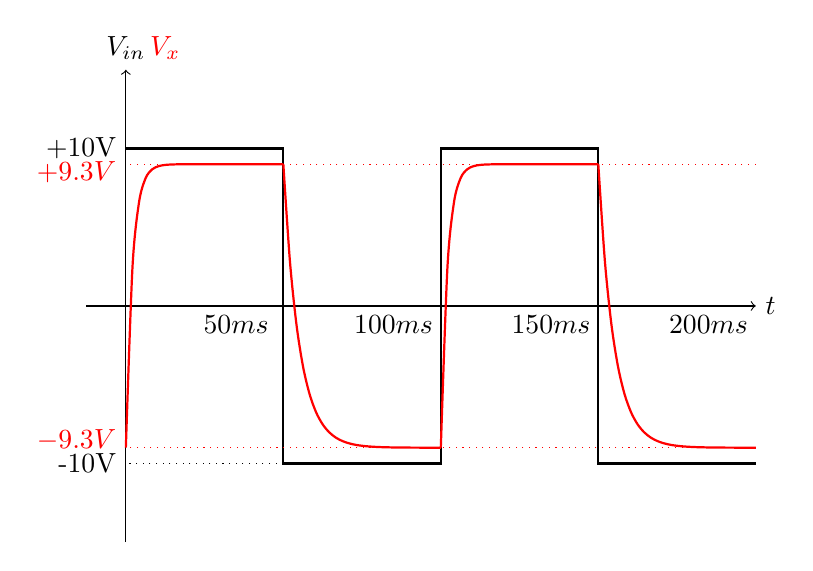
\begin{tikzpicture}
      \draw[->] (-0.5,0) -- (8,0) node[right] {$t$};
      \draw[->] (0,-3) -- (0,3) node[above] {$V_{in}$};
      \draw(0.5,3) node[red,above] {$V_x$};
      \draw(1.4,0) node[below]{$50ms$};
      \draw(3.4,0) node[below]{$100ms$};
      \draw(5.4,0) node[below]{$150ms$};
      \draw(7.4,0) node[below]{$200ms$};
      \draw[thick](0,2) -- (2,2) -- (2,-2) -- (4,-2) -- (4,2) -- (6,2) -- (6,-2) -- (8,-2);
      \draw[dotted] (2,-2) -- (0,-2);
      \draw[red,dotted] (8,-1.8) -- (0,-1.8);
      \draw[red,dotted] (8,1.8) -- (0,1.8);
      \draw(0,1.7) node[red,left]{$+9.3V$};
      \draw(0,-1.7) node[red,left]{$-9.3V$};
      \draw(0,2) node[left]{+10V};
      \draw(0,-2) node[left]{-10V};
      \draw[domain=0:2,smooth,variable=\x,thick,red] plot ({\x},{1.8-3.6*e^(-12*\x)});
      \draw[domain=2:4,smooth,variable=\x,thick,red] plot ({\x},{-1.8+3.6*e^(5*(2-\x))});
      \draw[domain=4:6,smooth,variable=\x,thick,red] plot ({\x},{1.8-3.6*e^(12*(4-\x))});
      \draw[domain=6:8,smooth,variable=\x,thick,red] plot ({\x},{-1.8+3.6*e^(5*(6-\x))});
    \end{tikzpicture}
\end{figure}


\clearpage
\textbf{2) Dissipazione potenza Diodi}
\begin{center}
    \begin{circuitikz}
        \draw (-4,6)  to[american voltage source, v^<= $V_{IN}$] (-4,0) node[ground] {};
        \draw(2,6)    to[short, -*] (0,6) to[short] (0,6) to[R,l_=$R_3$] (-4,6);
        \draw(0,4)    to[diode,i=$i_{D1}$,l_=$D_1$] (0,6);
        \draw(2,6)    to[diode,i=$i_{D2}$,l=$D_2$] (2,4);
        \draw(-0.5,6) to[open,v=$V_{D1}$] (-0.5,4);
        \draw(3,4)    to[open,v=$V_{D2}$] (3,6);
        \draw(0,4)    to[R,l=$R_1$] (0,2);
        \draw(0,2)    to[short, *-*] (2,2);
        \draw(2,4)    to[R,l=$R_2$] (2,2);
        \draw(0,2)    to[short] (0,0)  node[ground]{} (0,0);
        \draw(2,2)    to[C,l=$C_2$] (2,0)  node[ground]{} (2,0);
        \draw(2,2) node[right]{$V_x$};
    \end{circuitikz}
\end{center}

Il condensatore e' cortocircuitato a massa quindi

\begin{center}
    \begin{circuitikz}
        \draw (-4,6)  to[american voltage source, v^<= $V_{IN}$] (-4,1) node[ground] {};
        \draw(2,6)    to[short, -*] (0,6) to[short] (0,6) to[R,l_=$R_3$] (-4,6);
        \draw(0,4)    to[diode,i=$i_{D1}$,l_=$D_1$] (0,6);
        \draw(2,6)    to[diode,i=$i_{D2}$,l=$D_2$] (2,4);
        \draw(-0.5,6) to[open,v=$V_{D1}$] (-0.5,4);
        \draw(3,4)    to[open,v=$V_{D2}$] (3,6);
        \draw(0,4)    to[R,l=$R_1$] (0,2);
        \draw(2,4)    to[R,l=$R_2$] (2,2);
        \draw(0,2)    to[short, -] (2,2);
        \draw(1,2)    to[short, *-] (1,1) node[ground]{} (1,1);
        \draw(1,2) node[above]{$V_x$};
    \end{circuitikz}
\end{center}

\[V_x(t) = 0V\]
La potenza dissipata dai diodi e':
\[P_D = V_\gamma i_D\]
quindi dissipera' piu' potenza il diodo su cui circola piu' corrente.
\[i_{D2} = \frac{V_{IN} - V_\gamma}{R_3 + R_2} \]
\[i_{D1} = \frac{V_{IN} - V_\gamma}{R_3 + R_1} \]
\[i_{D2} \ge i_{D1}  \Leftrightarrow  R_2 \le R_1\]
Quindi $D_2$ e' il diodo che dissipa piu' potenza a parita' di tempo acceso.

\[P_{D2} = V_\gamma i_{D2} = V_\gamma \frac{V_{IN} - V_\gamma}{R_3 + R_2}\]
e poiche' il duty-cycle e' il 50\% la potenza media per periodo e':

\[P_{D2} = D_{cycle} V_\gamma i_{D2} =\frac{1}{2} V_\gamma \frac{V_{IN} - V_\gamma}{R_3 + R_2} = 21.7mW\]

\clearpage
\textbf{3) Grafico della tensione $V_x$}
\begin{center}
    \begin{circuitikz}
        \draw (-4,6)  to[american voltage source, v^<= $V_{IN}$] (-4,0) node[ground] {};
        \draw(2,6)    to[short, -*] (0,6) to[short] (0,6) to[R,l_=$R_3$] (-4,6);
        \draw(0,4)    to[diode,i=$i_{D1}$,l_=$D_1$] (0,6);
        \draw(2,6)    to[diode,i=$i_{D2}$,l=$D_2$] (2,4);
        \draw(-0.5,6) to[open,v=$V_{D1}$] (-0.5,4);
        \draw(3,4)    to[open,v=$V_{D2}$] (3,6);
        \draw(0,4)    to[R,l=$R_1$] (0,2);
        \draw(0,2)    to[short, *-*] (2,2);
        \draw(2,4)    to[R,l=$R_2$] (2,2);
        \draw(0,2)    to[R,l=$R$] (0,0)  node[ground]{} (0,0);
        \draw(2,2)    to[C,l=$C_2$] (2,0)  node[ground]{} (2,0);
        \draw(2,2) node[right]{$V_x$};
    \end{circuitikz}
\end{center}

In questo caso il condensatore si scarica costantemente attraverso $R$,
la tabella di polarizzazione dei diodi e' uguale a prima:
\begin{tabular}{c | c c}
    $V_{IN}$ & $D_1$ & $D_2$\\
    \hline
    $V_{IN} \ge V_\gamma = 0.7V$ & On & Off\\
    $0.7V \ge V_{IN} \ge -0.7V$ & Off & Off\\
    $-0.7V \ge V_{IN} $ & Off & On
\end{tabular}

\textbf{Quando entrambi i diodi son spenti} il condensatore e' appeso quindi non puo' scaricarsi e quindi la tensione $V_x$ rimane costante, ma poiche' $V_{IN}$ e' un onda quadra il tempo per cui $0.7V \ge V_{IN} \ge -0.7V$ e' trascurabile rispetto al periodo quindi possiamo ignorare questo punto di funzionamento ed ottenere una buona approssimazione.

\textbf{Quindi con $D_1$ Spento e $D_2$ Acceso}
\[\tau_c = C (R // (R2 + R3)) = 750\mu s\]
e poiche' 
\[T_a \approx 5 \tau_c = 3.75ms \le \frac{1}{f_{in}} = 100ms\]
allora il condensatore arriva a caricarsi completamente a :
\[V_x = (V_{IN} - V_\gamma ) \frac{R}{R + R_2 + R_3} = 4.65V \]

\textbf{Quindi con $D_1$ Acceso e $D_2$ Spento}
\[\tau_s = C (R // (R1 + R3)) = 1ms\]
e poiche' 
\[T_a \approx 5 \tau_s = 5ms \le \frac{1}{f_{in}} = 100ms\]
allora il condensatore arriva a caricarsi completamente a :
\[V_x =(V_{IN} - V_\gamma ) \frac{R}{R + R_1 + R_3}= -3.1V \]
Quindi $V_x$ sara' una onda quadra coi fronti di salita e discesa smussati con dinamica $[-3.1V,+4.6V]$ di pari frequenza al segnale in ingresso, e poiche' $\tau_c \le \tau_s$ i fronti di salita saranno piu' ripidi di quelli di discesa.

\begin{figure}[H]
    \center
    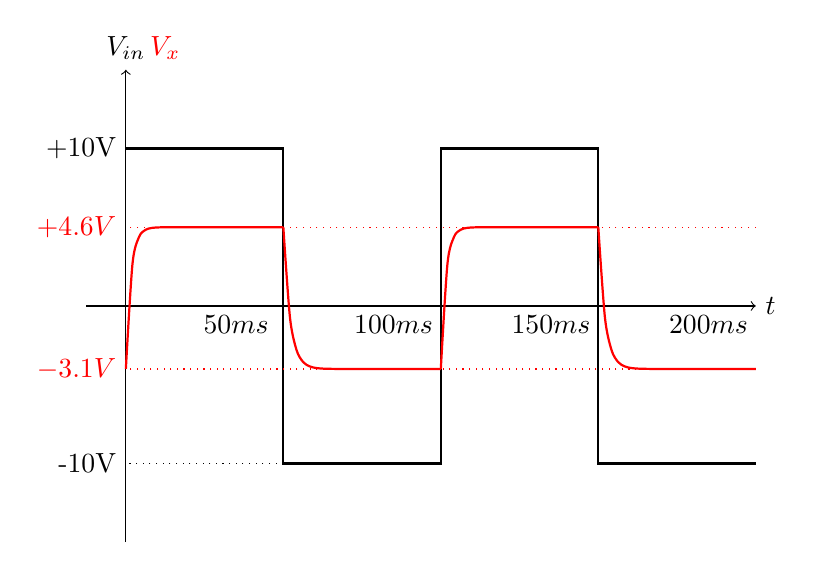
\begin{tikzpicture}
      \draw[->] (-0.5,0) -- (8,0) node[right] {$t$};
      \draw[->] (0,-3) -- (0,3) node[above] {$V_{in}$};
      \draw(0.5,3) node[red,above] {$V_x$};
      \draw(1.4,0) node[below]{$50ms$};
      \draw(3.4,0) node[below]{$100ms$};
      \draw(5.4,0) node[below]{$150ms$};
      \draw(7.4,0) node[below]{$200ms$};
      \draw[thick](0,2) -- (2,2) -- (2,-2) -- (4,-2) -- (4,2) -- (6,2) -- (6,-2) -- (8,-2);
      \draw[dotted] (2,-2) -- (0,-2);
      \draw[red,dotted] (8,-0.8) -- (0,-0.8);
      \draw[red,dotted] (8,1) -- (0,1);
      \draw(0,1) node[red,left]{$+4.6V$};
      \draw(0,-0.8) node[red,left]{$-3.1V$};
      \draw(0,2) node[left]{+10V};
      \draw(0,-2) node[left]{-10V};
      \draw[domain=0:2,smooth,variable=\x,thick,red] plot ({\x},{1-1.8*e^(-16*\x)});
      \draw[domain=2:4,smooth,variable=\x,thick,red] plot ({\x},{-0.8+1.8*e^(12*(2-\x))});
      \draw[domain=4:6,smooth,variable=\x,thick,red] plot ({\x},{1-1.8*e^(16*(4-\x))});
      \draw[domain=6:8,smooth,variable=\x,thick,red] plot ({\x},{-0.8+1.8*e^(12*(6-\x))});
    \end{tikzpicture}
\end{figure}



\end{document}


















